\documentclass{beamer}

\mode<presentation>
{
  \usetheme{Berkeley}
  \usecolortheme{crane}

  \setbeamercovered{transparent}
  % or whatever (possibly just delete it)
}


\usepackage[english]{babel}
% or whatever

\usepackage[latin1]{inputenc}
% or whatever

\usepackage{times}
\usepackage[T1]{fontenc}
% Or whatever. Note that the encoding and the font should match. If T1
% does not look nice, try deleting the line with the fontenc.
\usepackage{natbib} 
\usepackage{minted}
\usepackage{graphicx}

\graphicspath{{assets/figures/}}
\DeclareGraphicsExtensions{.pdf,.png,.jpg}

\title{DeeBee}
\subtitle{Implementation of a Relational Database Query-Processing System}

\author{Hawk Weisman}

\institute[Allegheny College] % (optional, but mostly needed)
{Department of Computer Science\\Allegheny College
}

\date{December 8th, 2014}

\subject{Compilers, Databases}
% This is only inserted into the PDF information catalog. Can be left
% out. 




% Delete this, if you do not want the table of contents to pop up at
% the beginning of each subsection:
\AtBeginSubsection[]
{
  \begin{frame}<beamer>{Outline}
    \tableofcontents[currentsection,currentsubsection]
  \end{frame}
}


% If you wish to uncover everything in a step-wise fashion, uncomment
% the following command: 

%\beamerdefaultoverlayspecification{<+->}
%\addbibresource{assets/final.bib}

\begin{document}

\begin{frame}
  \titlepage
\end{frame}

\begin{frame}{Outline}
  \tableofcontents
  % You might wish to add the option [pausesections]
\end{frame}


% Structuring a talk is a difficult task and the following structure
% may not be suitable. Here are some rules that apply for this
% solution: 

% - Exactly two or three sections (other than the summary).
% - At *most* three subsections per section.
% - Talk about 30s to 2min per frame. So there should be between about
%   15 and 30 frames, all told.

% - A conference audience is likely to know very little of what you
%   are going to talk about. So *simplify*!
% - In a 20min talk, getting the main ideas across is hard
%   enough. Leave out details, even if it means being less precise than
%   you think necessary.
% - If you omit details that are vital to the proof/implementation,
%   just say so once. Everybody will be happy with that.
\section{Introduction}
\begin{frame}{Introduction}
\begin{itemize}
  \item Query processing:  \pause
  \begin{itemize}
    \item An application of many concepts from compilers \pause
    \item Vital to today's world (databases are everywhere)  \pause
  \end{itemize}
  \item DeeBee: \pause
  \begin{itemize}
    \item A very small relational database (\textless 1500 LoC) \pause
    \item Implements a subset of the Structured Query Language  \pause
    \item For educational purposes only (don't use this in production)  \pause
    \item Written in the Scala programming language 
  \end{itemize}
  \end{itemize}
\end{frame}

\section{Background}

\subsection{Relational Databases}

\begin{frame}{What is a relational database?}
\begin{itemize}
 	 \item ``The primary data model for commercial data-processing applications.''~\citep[39]{silberschatz2010database} \pause
 	 \item A database consists of multiple tables of values, called \alert{relations}~\citep{silberschatz2010database,harrington2009relational,garcia2000database} \pause
 	 \item A relation consists of:~\citep{silberschatz2010database,harrington2009relational,garcia2000database} \pause
  \begin{itemize}
   		 \item a set of rows, or \alert{tuples}
       \item a set of columns, or \alert{attributes}
  	\end{itemize}  \pause
  	\item So how does this relate to compilers?
  \end{itemize}
\end{frame}

\subsection{Query Languages}

\begin{frame}{What is a query language?}
  \begin{itemize}
  \item Users and client software interact with databases through \alert{query languages}~\citep{silberschatz2010database,harrington2009relational,garcia2000database}  \pause
  \item These are \alert{domain-specific languages} for accessing and modifying the database  \pause
  \item Query languages are \alert{declarative} rather than \alert{imperative}~\citep{silberschatz2010database,harrington2009relational,garcia2000database}  \pause
  \item Just like other programming languages, query languages must be parsed, analyzed, and compiled or interpreted.~\citep{silberschatz2010database,harrington2009relational,garcia2000database}
  \end{itemize}
\end{frame}

\begin{frame}{SQL}
\begin{itemize}
  \item SQL is the \alert{Structured Query Language}.  \pause
  \item It is the query language used by most modern RDBMSs  \pause
  \item SQL consists of two components:  \pause
    \begin{itemize}
      \item \alert{Data definition language} (DDL): defines the structure of the database~\citep{silberschatz2010database,harrington2009relational} 
      \begin{itemize}  \pause
        \item creating and deleting tables
        \item adding relationships between tables
        \item et cetera
        \end{itemize}
      \item \alert{Data manipulation language} (DML): accesses and modifies data stored in the database~\citep{silberschatz2010database,harrington2009relational}  \pause
      \begin{itemize}
        \item selecting rows
        \item adding, deleting, and modifying rows
        \item et cetera
      \end{itemize} \pause
    \end{itemize} 
    \item SQL = DDL + DML
\end{itemize}
\end{frame}

\begin{frame}[fragile]{SQL Examples}
\begin{example}[SQL CREATE TABLE statement (schema)]
    \begin{minted}[gobble=8,fontsize=\footnotesize]{SQL}
        CREATE TABLE Writers (
            id            INTEGER NOT NULL PRIMARY KEY,
            first_name           VARCHAR(15) NOT NULL,
            middle_name          VARCHAR(15),
            last_name            VARCHAR(15) NOT NULL,
            birth_date           VARCHAR(10) NOT NULL,
            death_date           VARCHAR(10),
            country_of_origin    VARCHAR(20) NOT NULL
        );
\end{minted}
  \end{example}
\end{frame}

\begin{frame}[fragile]{SQL Examples}
\begin{example}[SQL SELECT statement]
    \begin{minted}[gobble=8,fontsize=\footnotesize]{SQL}
        SELECT * FROM test;
        SELECT test1, test2 FROM test;
        SELECT * FROM test WHERE test1 = 9 AND test2 = 5;
        SELECT * FROM test LIMIT 5;
    \end{minted}
  \end{example} \pause
  \begin{example}[SQL DELETE statement]
    \begin{minted}[gobble=8,fontsize=\footnotesize]{SQL}
        DELETE FROM test WHERE test2 > 3 LIMIT 100;
    \end{minted}
  \end{example}  \pause
    \begin{example}[SQL INSERT statement]
    \begin{minted}[gobble=8,fontsize=\footnotesize]{SQL}
        INSERT INTO test VALUES (
          1, 'a string', 2, 'another string'
        );
        \end{minted}
  \end{example}
\end{frame}

\subsection{Query Processing}

\begin{frame}{Steps in Query Evaluation}
\begin{figure}
  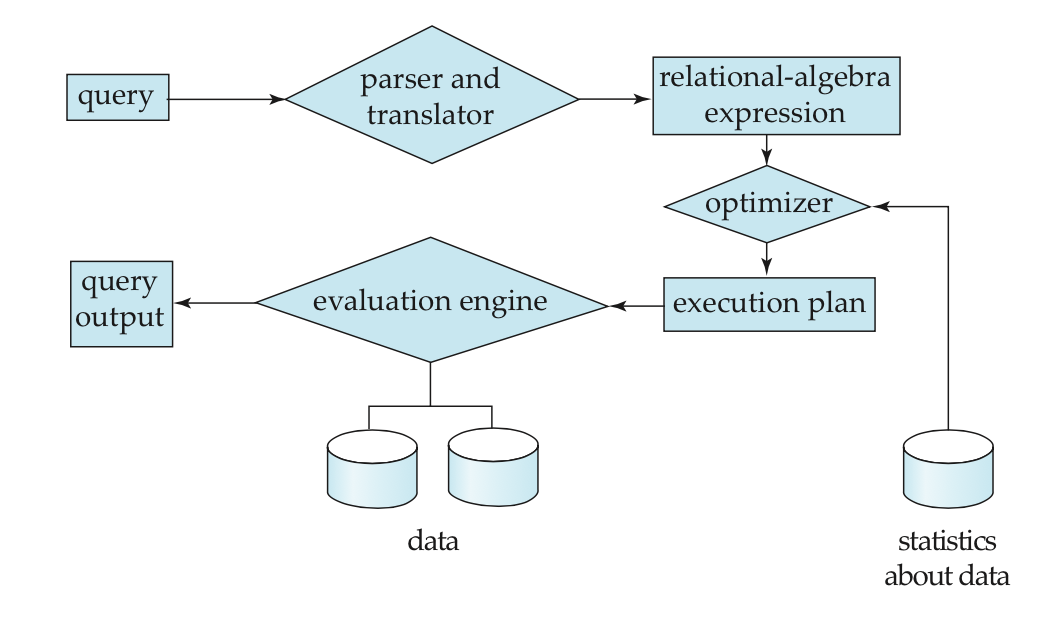
\includegraphics[width=\linewidth]{QueryProcessing}
  \caption{Steps in query processing~\citep[583]{silberschatz2010database}.}
  
\end{figure}
\end{frame}

\begin{frame}{Query Processing}
  \begin{itemize}
    \item A query processor is essentially a compiler!  \pause
    \item Some stages in the query evaluation process correspond directly to those in compilation: \pause
    \begin{itemize}
      \item Parsing \pause
      \item Semantic analysis \pause
      \item IR generation (Relational algebra expression)  \pause
      \item Optimization  \pause
    \end{itemize}
  \end{itemize}
\end{frame}



\section{DeeBee}

\subsection{Design}
\begin{frame}{Design Overview} 
  \begin{itemize}
    \item DeeBee implements a subset of SQL \pause
    \item Chosen to balance functionality with time constraints \pause
    \begin{itemize}
      \item \texttt{SELECT} statements  \pause
        \begin{itemize}
            \item Projections (\texttt{SELECT a, b FROM ...})  \pause
            \item Filtering by predicates (\texttt{SELECT * FROM table WHERE ...})  \pause
            \item Nested predicates  (\texttt{WHERE ... AND ... })  \pause
            \item \texttt{LIMIT} clauses  \pause
            \item No \texttt{JOIN}s  \pause
          \end{itemize}
      \item \texttt{INSERT} statements  \pause
      \item \texttt{DELETE} statements  \pause
        \begin{itemize}
          \item \texttt{WHERE} and \texttt{LIMIT} clauses  \pause
          \item Same implementation as \texttt{SELECT}  \pause
        \end{itemize}
      \item \texttt{CREATE TABLE} and \texttt{DROP TABLE} statements  \pause
      \begin{itemize}
        \item No \texttt{CHECK} constraints  \pause
        \item No \texttt{TRIGGER}s 
      \end{itemize}
    \end{itemize}
  \end{itemize}
\end{frame}

\begin{frame}{Architecture}
  \begin{itemize}
    \item The \alert{actors} model~\citep{gupta2012akka,haller2012integration,agha1985actors}  \pause
    \begin{itemize}
      \item A construct for concurrent programming \pause
      \item Actors communicate through \alert{message passing} \pause
      \item Messages are: \pause
      \begin{itemize}
        \item Immutable  \pause
        \item Asynchronous \pause
        \item Anonynous (decoupled) \pause
      \end{itemize}
      \item Actors enqueue recieved messages and respond to them in order \pause
    \end{itemize}
    \item {Essentially, an actor is a \alert{state machine} with a \alert{mailbox}} \pause
    \item Advantages:  \pause
    \begin{itemize}
      \item Fault tolerance (loose coupling)  \pause
      \item Scalability  \pause
      \item Concurrency   \pause
      \item Event-driven (good for databases)  \pause
    \end{itemize}
    \item In Scala, the Actors model is provided by the \alert{Akka} framework
  \end{itemize}
\end{frame}

\begin{frame}{Architecture}
  \begin{itemize}
    \item In DeeBee: \pause
    \begin{itemize}
      \item tables 
      \item databases 
      \item frontends (connections into the database)  \pause
    \end{itemize}
    \item ...are all represented by actors  \pause
    \item A database actor is responsible for:  \pause
    \begin{itemize}
      \item dispatching queries to its' tables  \pause
      \item sending query results to the querying entity  \pause
      \item creating and deleting table actors  \pause
  \end{itemize}
    \item A table actor is responsible for:  \pause
    \begin{itemize}
      \item recieving queries  \pause
      \item (possibly) updating its' state  \pause
      \item responding with query results or errors 
    \end{itemize}
  \end{itemize}
\end{frame}

\begin{frame}{Query Processing}
\begin{itemize}
  \item SQL queries are internally represented using an \alert{abstract syntax tree} (AST)  \pause
  \item Connection actors recieve \alert{query strings}, parse them, and send the AST to the database actor  \pause
  \item Database actor either:  \pause
    \begin{itemize}
      \item processes DDL queries by creating/deleting tables  \pause
      \item dispatches DML queries to the target child table  \pause
    \end{itemize}
    \item Queries are \alert{interpreted} (not compiled) against a context 
\end{itemize}
\end{frame}

\subsection{Implementation}
\subsubsection{Query Parsing}
\begin{frame}{Parser Combinators}
  \begin{itemize}
  \item DeeBee's query processor parses queries using \alert{combinator parsing}~\citep{moors2008parser,swierstra2001combinator,fokker1995functional,odersky2008programming}  \pause
  \item This is a functional-programming approach to text parsing  \pause
  \begin{itemize}
    \item A \alert{parser} is a function which accepts some strings and rejects others  \pause
    \item A \alert{parser-combinator} is a higher-order function which takes as input two or more parsers and returns combined parser  \pause
    \item By repeatedly combining simpler parsers into more complex ones, a \alert{recursive-descent parser} can be created  \end{itemize}
  \end{itemize}
\end{frame}

\begin{frame}[fragile]{Parser Combinators in Scala}
  \begin{itemize}
    \item Scala's parsing library follows the philosophy of \alert{embedded DSLs}~\citep{ghosh2010dsls,hofer2008polymorphic,moors2008parser,odersky2008programming}  \pause
    \item It allows parsers to be specified in \alert{BNF-like} syntax  \pause
    \begin{example}[Combinator Parsing in Scala]
    \begin{minted}[
    gobble=8,
    %firstline=115,
    %lastline=121,
    fontsize=\footnotesize
    ]{scala}
        def inPlaceConstraint: Parser[Constraint] = 
          ("not" ~ "null") ^^^ Not_Null
            | ("primary" ~ "key") ^^^ Primary_Key
            | "unique" ^^^ Unique
    \end{minted}
    \end{example}

  \end{itemize}
\end{frame}

\begin{frame}[fragile]{Packrat Parsing}
  \begin{itemize}
    \item \alert{Packrat parsers} add a memoization facility~\cite{jonnalagedda2009packrat,frost2008parser}  \pause
    \begin{itemize}
      \item Guarantees unlimited lookahead and linear parse time  \pause
      \item Allows parsing of left-recursive grammars  \pause
    \end{itemize}
    \item Parser functions are replaced by lazily-evaluated values  \pause
        \begin{example}[Combinator Parsing in Scala]
    \begin{minted}[
    %firstline=115,
    %lastline=121,
    fontsize=\footnotesize
    ]{scala}
lazy val expression: P[Expr[_]] = 
  ("(" ~> comparison <~ ")") ^^{
    case c: Comparison => new ParenComparison(c)
  }
    | comparison
    | literal
    | identifier
lazy val comparison: P[Comparison] = 
  expression ~ operator ~ expression ^^ {
    case lhs ~ op ~ rhs => Comparison(lhs, op, rhs)
  }  
    \end{minted}
    \end{example}
  \end{itemize}
\end{frame}
\subsection{Parsing Demo}
\subsection{Query Processing}
\begin{frame}{Query Processing}
  \begin{itemize}
    \item DeeBee queries are \alert{interpreted} \pause
    \item Interpretation is \alert{contextualized} against a database \pause
    \begin{itemize}
      \item \alert{Type checking} \pause
      \begin{itemize}
        \item In a compiler, context is preceeding program statements \pause
        \item In DBMS, context is the schema of the target table \pause
      \end{itemize}
      \item \alert{Predicate interpretation} \pause
      \begin{itemize}
        \item Convert AST nodes to Scala partial functions \pause
        \item Nested predicates are constructed from leaves to roots \pause
      \end{itemize}
      \item \alert{Constraints validation} \pause
      \begin{itemize}
        \item Ensure queries don't violate table constraints \pause
        \item Uniqueness \pause
        \item Not null \pause
        \item Type constraints \pause
        \item Eventually, this will be deferrable for transaction processing
      \end{itemize}
    \end{itemize}
  \end{itemize}
\end{frame}
\subsection{Query Processing Demo}


% All of the following is optional and typically not needed. 
\appendix
\section<presentation>*{\appendixname}
\subsection<presentation>*{References}

\begin{frame}[allowframebreaks]
        \frametitle{References}
        %\nocite{*} 
\bibliography{assets/final}{}
\bibliographystyle{plain}
\end{frame}

\end{document}


